\chapter{Introduction} \label{chap:intro}
\section{Why underwater?}
Manhood has managed to conquer variety of environments. At some point, humans could walk on the moon, send expeditions to cold or remote areas in different corners of the planet. Seabed embraces the largest part of the Earth's surface. Deep ocean world is a harsh environment with many discoveries yet to be revealed. Robots have potential to help in achieving those discoveries. 
\section{Localization - Where the Robot Is?}
One of the important features of the autonomous underwater vehicle is being capable of localising itself within an environment - to estimate its metric position and orientation in three dimensional space. Knowing where it actually is enables further tasks of an autonomous robot such as path tracking or various manipulation tasks. Therefore, it has the same role as parts of human brain devoted to the navigation.  

The main topic of the thesis is localisation of an autonomous underwater vehicle. Localisation essentially deals with the problem of estimating the position and orientation of the vehicle with respect to the defined reference system. Simply, answering where the robot is. Basic instrument in accomplishing the localisation is the sensor set. Sensory system is used to supply the localisation algorithm with the feedback on vehicle movement, control or state of the surrounding environment and its relation with the vehicle. One of the difficulties when interpreting the sensory information is the very nature of the measurement - noisy and uncertain. Majority of the measurements obtained from sensors are based on evaluation of the distance in water environment. Many conditions can influence the performance of the localisation, including the very beginning: whether we can make some estimate on the initial position or not \cite{ribas10}. 

%Localization can alternatively be carried out by analysing the pose possibilities and choosing the one that better correlates to measurements or the map. Such methods are Monte Carlo localization and Markov localization. The other approach, a set of hypotheses for coupling together the sensor measurements and the map features. These hypotheses are ranked depending on number of consistent matches where the one with highest ranking is defining the position. This can be a costly process, therefore a number of methods deals with optimization of it. 
\section{Autonomous underwater vehicle (AUV)}
Different sorts of underwater robots have been developed throughout recent decades of research. They all have various performance capabilities, costs, accuracy, power consumption characteristics. The algorithm presented in this thesis was applied on Ocean System Lab's (\url{http://osl.eps.hw.ac.uk/}) torpedo-shaped Nessie vehicle (figure ~\ref{fig:nessie6}) that belongs to special-task AUV category combining together FOG-based Inertial Navigation System, DVL and LBL sensoring for aiding navigation (Chapter ~\ref{chap:sensors}). The architecture of the vehicle and its system capabilities are flexible on number and types of sensors employed leaving space for additional equipment to assist in missions, or improve the current navigation with already existing devices, such as forward or downward looking cameras. 
\begin{figure}%[htp]
\centering
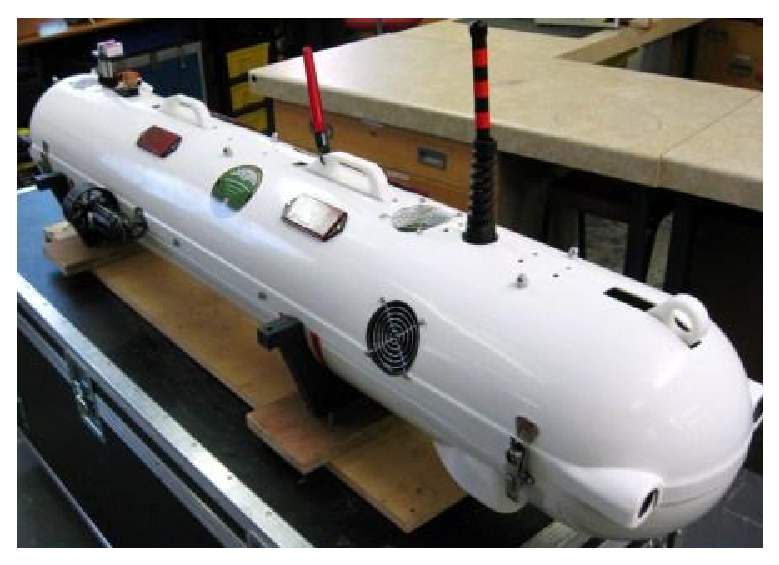
\includegraphics[width=0.5\linewidth]{intro/fig/nessie6.eps}
\caption{Nessie AUV design.}
\label{fig:nessie6}
\end{figure} 

\section{Contribution of the thesis}
Thesis is reporting the application of Extended Kalman Filter for localisation of the above mentioned Nessie AUV in an unstructured environment. The concept of sensor fusion was explained. The main contribution is the implementation of an EKF estimator adopted to work on a real underwater vehicle with real-time signals received from sensors. Furthermore, design of the estimator requires establishing a prediction model. Five d.o.f. model of the vehicle dynamics was introduced to take the role of the prediction. Apart from the algorithm-level investigation, following work examines the problem from the perspective of engineering a successful AUV navigation in general. The issue of accurate heading and the outliers in absolute position measurement  was analysed. Unscented Kalman Filter was implemented as an attempt to improve the performance and compensate for the shortcomings of the EKF. Eventually, simulations and some real scenarios were carried out resulting in analysis of the performance, advantages and disadvantages of the method. 
%Idea of blending together sensor measurements can be exploited in different situations.
\section{Thesis outline}
The first chapter \S~\ref{chap:problem-def} introduces the task of robot navigation. Chapter \S~\ref{chap:capabilities} explores the possible methods to navigate the robot and gives an overview of the literature that covers AUV navigation. A digression on theory of nonlinear filtering and Kalman Filtering algorithms such as was EKF and UKF was included in the chapter. Since the investigated navigation task relies on sensory data, a short overview on vehicle sensors is given in Chapter \S~\ref{chap:sensors}. Methodology describing the details of the implementation was shown in Chapter \S~\ref{chap:methodology}. Finally, results obtained from the real missions were given in \S~\ref{chap:results}, with concluding remarks placed in last section \S~\ref{chap:conclusions}.
%%\subsection{Paper}
%%The manuscript should be in A4 size, and the printed paper should
%%be of at least 70 gsm.
%%
%%\subsection{Font and margins}
%%Thesis should be printed on both sides of the paper. Use no less
%%than 1.5 spacing, with quotations and notes single-spaced.
%%Regarding \textbf{Character size}, not less than 2.0mm for
%%capitals and 1.5mm for x-height (the height of a lower-case x). Us
%%a serif font (i.e. Times) between 10 and 12 points. Use consistent
%%and clear fonts through all the document.
%%
%%The text layout should be approximately as follows:
%%
%%\begin{itemize}
%%    \item $4cm$ binding margin
%%    \item $2cm$ head margin (top of page)
%%    \item $2.5cm$ fore-edge margin
%%    \item $4cm$ tail margin (bottom of page)
%%\end{itemize}
%%
%%\section{Title Page}
%%The title page should contain the title of thesis, authors name,
%%and at the foot of the page: the name of degree,  Your University,
%%and the year of presentation. Something like this:
%%
%%\vspace*{1cm}
%%\begin{center}
%%{\Large\bf MSc. Thesis example VIBOT\\} \vspace{2cm} {\large
%%Robert Mart\'i\\
%%\vspace{1cm}
%%Department of Computer Architecture and Technology \\
%%University of Girona}
%%
%%\end{center}
%%
%%\vspace{2cm}
%%\begin{center}
%%{\large A Thesis Submitted for the Degree of MSc Erasmus Mundus in
%%Vision and Robotics (VIBOT)\\ \vspace{0.3cm} $\cdot$ 2008 $\cdot$}
%%\end{center}
%%
%%
%%\subsection{References}
%%You can reference other authors by using the $cite command$
%%\cite{Pokorski:1998hr}. You are encouraged to use bib files and
%%let bibtex do the job for you.
